\documentclass[../main.tex]{subfiles}

\begin{document}

\chapter{Model Development}

\begin{modelchapter}

The following chapter details the process to develop a model for the fluctuation
strength sensation, based on \citeauthor{daniel1997psychoacoustical}'s roughness
model. The model will be analyzed in stages, where the changes needed to adapt
it to this particular case will be detailed. After that, a procedure to adjust
the parameters of the model is presented. Finally, the results of the
fluctuation strength model will be presented, and the limitations of the data
fitting will be addresed.

\section{Roughness Model}

\begin{figure}[!ht]
  \centering
  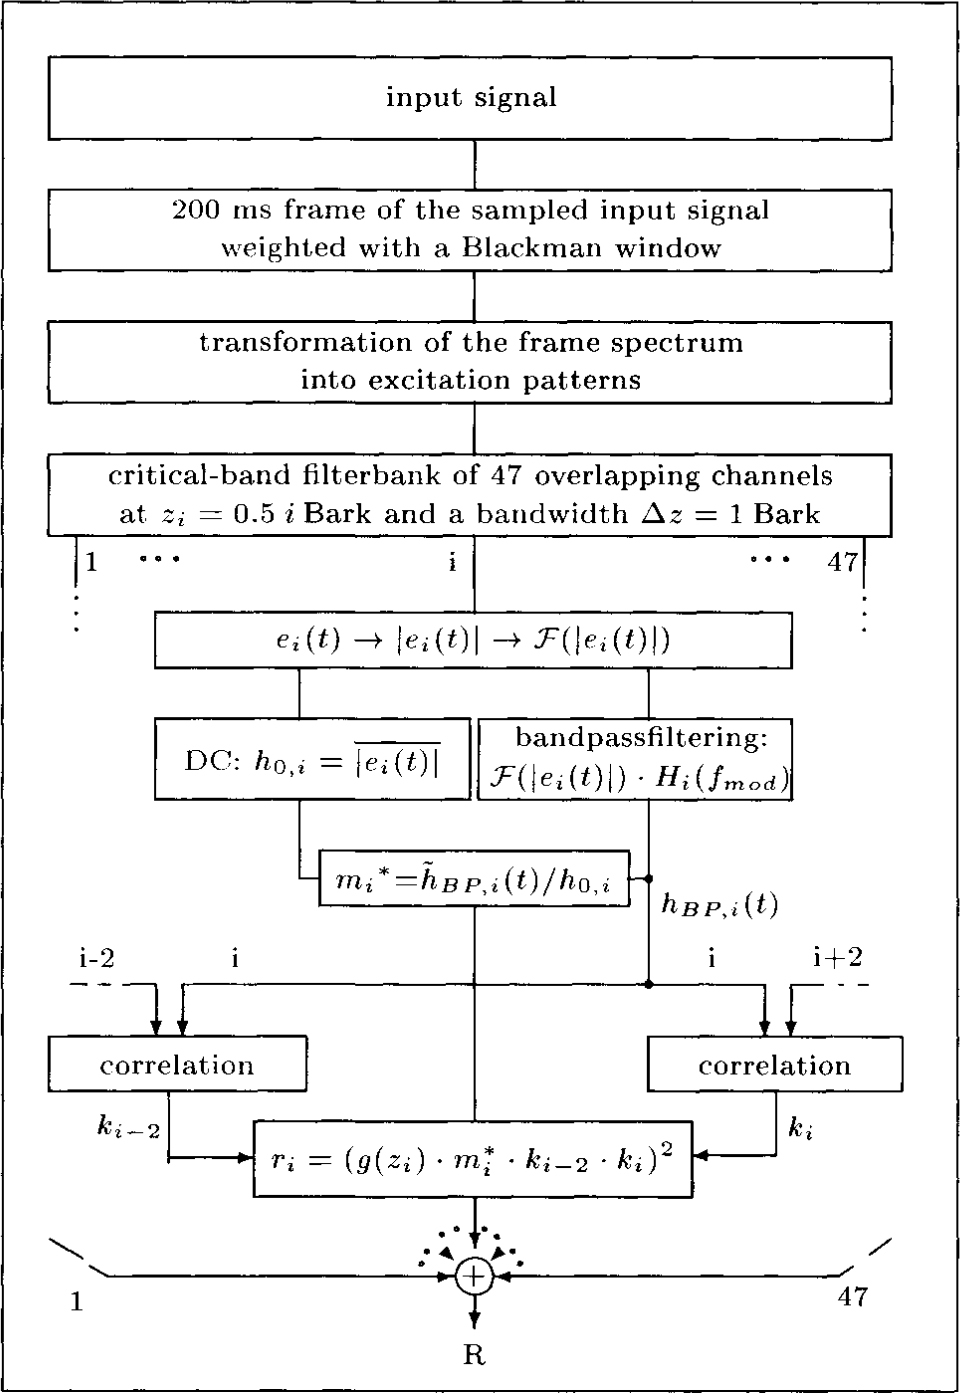
\includegraphics[height=8cm]{model}
  \caption{Caption here}
  \label{fig:figure1}
\end{figure}

\section{Procedure}




\section{Results}

\modelresultsfigure{am-fm}{modulation frequency}{AM}
\modelresultsfigure{am-fc}{center frequency}{AM}
\modelresultsfigure{am-spl}{sound pressure level}{AM}
\modelresultsfigure{am-md}{modulation depth}{AM}
\modelresultsfigure{fm-fm}{modulation frequency}{FM}
\modelresultsfigure{fm-fc}{center frequency}{FM}
\modelresultsfigure{fm-spl}{sound pressure level}{FM}
\modelresultsfigure{fm-df}{frequency deviation}{FM}


\end{modelchapter}

\end{document}
